%%%%%%%%%%%%%%%%%%%%%%%%%%%%%%%%%%%%%%%%%%%%%%%%%%%%%%%%%%%%%%%
\section{Electrons}\label{sec:electrons}
%%%%%%%%%%%%%%%%%%%%%%%%%%%%%%%%%%%%%%%%%%%%%%%%%%%%%%%%%%%%%%%
%
%%%%%%%%%%
\subsection{Electron reconstruction}\label{subsec:elereco}
%%%%%%%%%%

The electron reconstruction in CMS~\cite{Baffioni:2006cd} is based on the association of an energy deposit in the ECAL with a track reconstructed in the silicon tracker system.
Electrons lose energy primarily through bremsstrahlung when interacting with the tracker layers, and consequently they suffer from large energy losses.
Given the non-Gaussian properties of the energy loss distributions, the standard track reconstruction algorithm based on the KF is not appropriate
and leads in general to a reduced hit-collection efficiency, as well as to a poor estimation of track parameters. 
A better performance for electron reconstruction is achieved by using dedicated techniques that make use of information, not only from the tracker, but also from the ECAL, as described in the following.\\
%As electrons lose energy primarily through bremsstrahlung, large energy losses are common.
%About 35\% of electrons radiate more than 70\% of their initial energy before reaching ECAL.
%An important property of the electrons is their high probability of emitting a bremsstrahlung photon after interacting with one of the tracker layers.
%Electrons, being charged particles, can be reconstructed through the standard track reconstruction.  However,  as electrons lose energy primarily through bremsstrahlung,  rather than ion- ization,  large energy losses are common.  For example,  about 35\% of electrons radiate more than 70\% of their initial energy before reaching the electromagnetic calorimeter (ECAL) that surrounds the tracker.  The energy loss distribution is highly non-Gaussian, and therefore the standard Kalman filter, which is optimal when all variables have Gaussian uncertainties, is not appropriate. As a result, the efficiency and resolution of the standard tracking are not particularly good for electrons and therefore electron candidates are reconstructed using a combination of two techniques that make use of information, not only from the tracker, but also from the ECAL. 

The electron reconstruction starts by searching for clusters of energy in the ECAL.
As the electrons are degraded in energy, the effect of the magnetic field is to enhance the bending of their trajectories, resulting in a spread of irradiated photons along the $\phi$ coordinate.
To recover this radiated energy, ECAL superclusters are formed, by merging clusters of similar $\eta$ over some range of $\phi$.
Because of the different geometry of the detector in barrel and endcap, different clustering algorithms are used in different regions.
%Because of bremsstrahlung the electron energy usually spreads out over several crystals of the ECAL. 
%Bremsstrahlung photons emitted by the electrons strike, in general, the ECAL at $\eta$ values similar to that of the electron,
%but at different $\phi$. To recover this radiated energy, ECAL superclusters are formed, by merging clusters of similar $\eta$ over some range of $\phi$.
%Because of the different geometry of the detector in barrel and endcap, different clustering algorithms are used in different regions
%The first method [35] starts by searching for clusters of energy in the ECAL. The curvature
%of electrons in the strong CMS magnetic field means that bremsstrahlung photons emitted by
%the electrons will, in general, strike the ECAL at eta values similar to that of the electron, but
%at different azimuthal coordinates phi.  To recover this radiated energy, ECAL superclusters
%are formed, by merging clusters of similar eta over some range of f.  

For the electron track reconstruction two approaches are used.
In the first one, referred to as ``ECAL driven'', the supercluster energy and position, and the assumption that the electron originated near the center of the beam spot, are used to extrapolate the electron trajectory in the tracker. Tracker seeds compatible with the predicted trajectory are sought in the first or second layer of the pixel detector (and also in the TEC to improve efficiency in the forward region).
This method is designed for isolated electrons with $\pt > 5\GeV$.

%A ?tracker driven? approach, developped in the context of the PF algorithm, is also used and extends the electron track reconstruction for low momentum and non isolated electrons.
A second approach, referred to as ``tracker driven'', complements the electron track reconstruction,
especially for low-\pt or non isolated electrons, as well as for electrons in the barrel-endcap transition region. This method is developed as part of the particle-flow (PF) reconstruction algorithm~\cite{CMS-PAS-PFT-10-001,CMS-PAS-PFT-09-001} described in Section~\ref{subsec:jetsreco}.
It takes the standard track collection reconstructed with the KF algorithm and attempts to identify a subset of these tracks that are compatible with being electrons. 
Electrons that suffer only little bremsstrahlung loss can be identified by searching for tracks extrapolated to the ECAL that pass close to an ECAL PF cluster.
Electrons that suffer large bremsstrahlung loss can be identified by the fact that the fitted track will often have poor $\chi^2$ or few associated hits. 
The track seeds originally used to generate these electron-like tracks are retained.

The seed collections obtained by using these two methods are merged, and used to initiate electron track finding. 
This procedure is similar to that used in standard tracking, except that the $\chi^2$ threshold, used by the KF to decide whether a hit is compatible with a trajectory, is weakened. 
This is to accommodate tracks that deviate from their expected trajectory because of bremsstrahlung.

To obtain the best estimate of the track parameters, the final track fit is performed using a modified version of the KF method, called the Gaussian Sum Filter (GSF)~\cite{0954-3899-31-9-N01}.
The fractional energy loss of an electron, as it traverses a layer of material, follows a Bethe--Heitler distribution. 
This distribution is non-Gaussian, making it unsuitable for use in a conventional KF algorithm. 
The GSF technique solves this by approximating the Bethe--Heitler energy-loss distribution as the sum of several Gaussian  functions.
This method is then a generalization of the KF where the trajectory in each tracker layer is described by a weighted sum of KF components for which the energy loss follows a Gaussian law with a given width.
The propagation of each component is done separately from one layer to another and the weights are then updated given the measurement in the new site.
The allowed window to search for a hit in the next tracker layer is larger than for the usual KF track.
This procedure is iterated until the last tracker layer, unless no hit is found in two subsequent layers. A minimum of five hits is finally required to create a track.
A GSF electron candidate is finally built by associating an ECAL supercluster with a GSF track with compatible $\eta$ and $\phi$ positions.

The electron transverse energy \et is equal to the transverse energy of the correspondent ECAL energy deposit (or supercluster) $\et^\mathrm{SC}$, and defined as
$\et = E\sin\theta$, where $\theta$ is the polar angle of the supercluster (ST) relative to the beam axis,
and $E$ the energy measured in the supercluster. 

The performance of the GSF electron reconstruction are studied using a ``tag-and-probe'' (T\&P) method~\cite{Khachatryan:2010xn}.
The method uses a known SM resonance mass and decay (e.g. $\PZ\to\EE$) to select particles of the desired type and probe the efficiency of a particular selection criterion on those particles. In general the ``tag'' is an object that passes a set of very tight selection criteria designed to isolate the required particle type (in this case an electron, though the method is not strictly limited to this case). A generic set of the desired particle type (i.e. with potentially very loose selection criteria) known as ``probes'', is selected by pairing these objects with tags such that the invariant mass of the combination is consistent with the mass of the resonance. Combinatoric backgrounds are usually eliminated through a variety of background subtraction methods. The definition of the probe object depends on the specifics of the selection criterion being examined. The efficiency itself is measured by counting the number of ``probe'' particles that pass the desired selection criteria. It is found that the estimated efficiencies are almost insensitive to any specific definition of the tag. 
%which exploits Z/$\gamma^*\rightarrow$e$^+$e$^-$ events in data to estimate the reconstruction and selection efficiencies for signal electrons. The method requires one electron candidate, called the ``tag'', to satisfy tight selection requirements. Different criteria are tried to define the tag electron, and it is found that the estimated efficiencies are almost insensitive to any specific definition of the tag. 
The GSF electron reconstruction efficiency measured with this method is above 95\% for electrons in the ECAL barrel with $\et > 35\GeV$, as shown in Fig.~\ref{fig:el_reco_a}. Slightly lower efficiencies are obtained for electrons reconstructed in the ECAL endcaps (Fig.~\ref{fig:el_reco_b}). A good agreement is found between data and simulation, resulting in scale factors consistent with unity almost in the entire range. The performance are presented here for the electron reconstruction in Run~1 but similar results are obtained in CMS for Run~2.\\

\begin{figure}[!htb]
\centering
\subfigure[]{\label{fig:el_reco_a}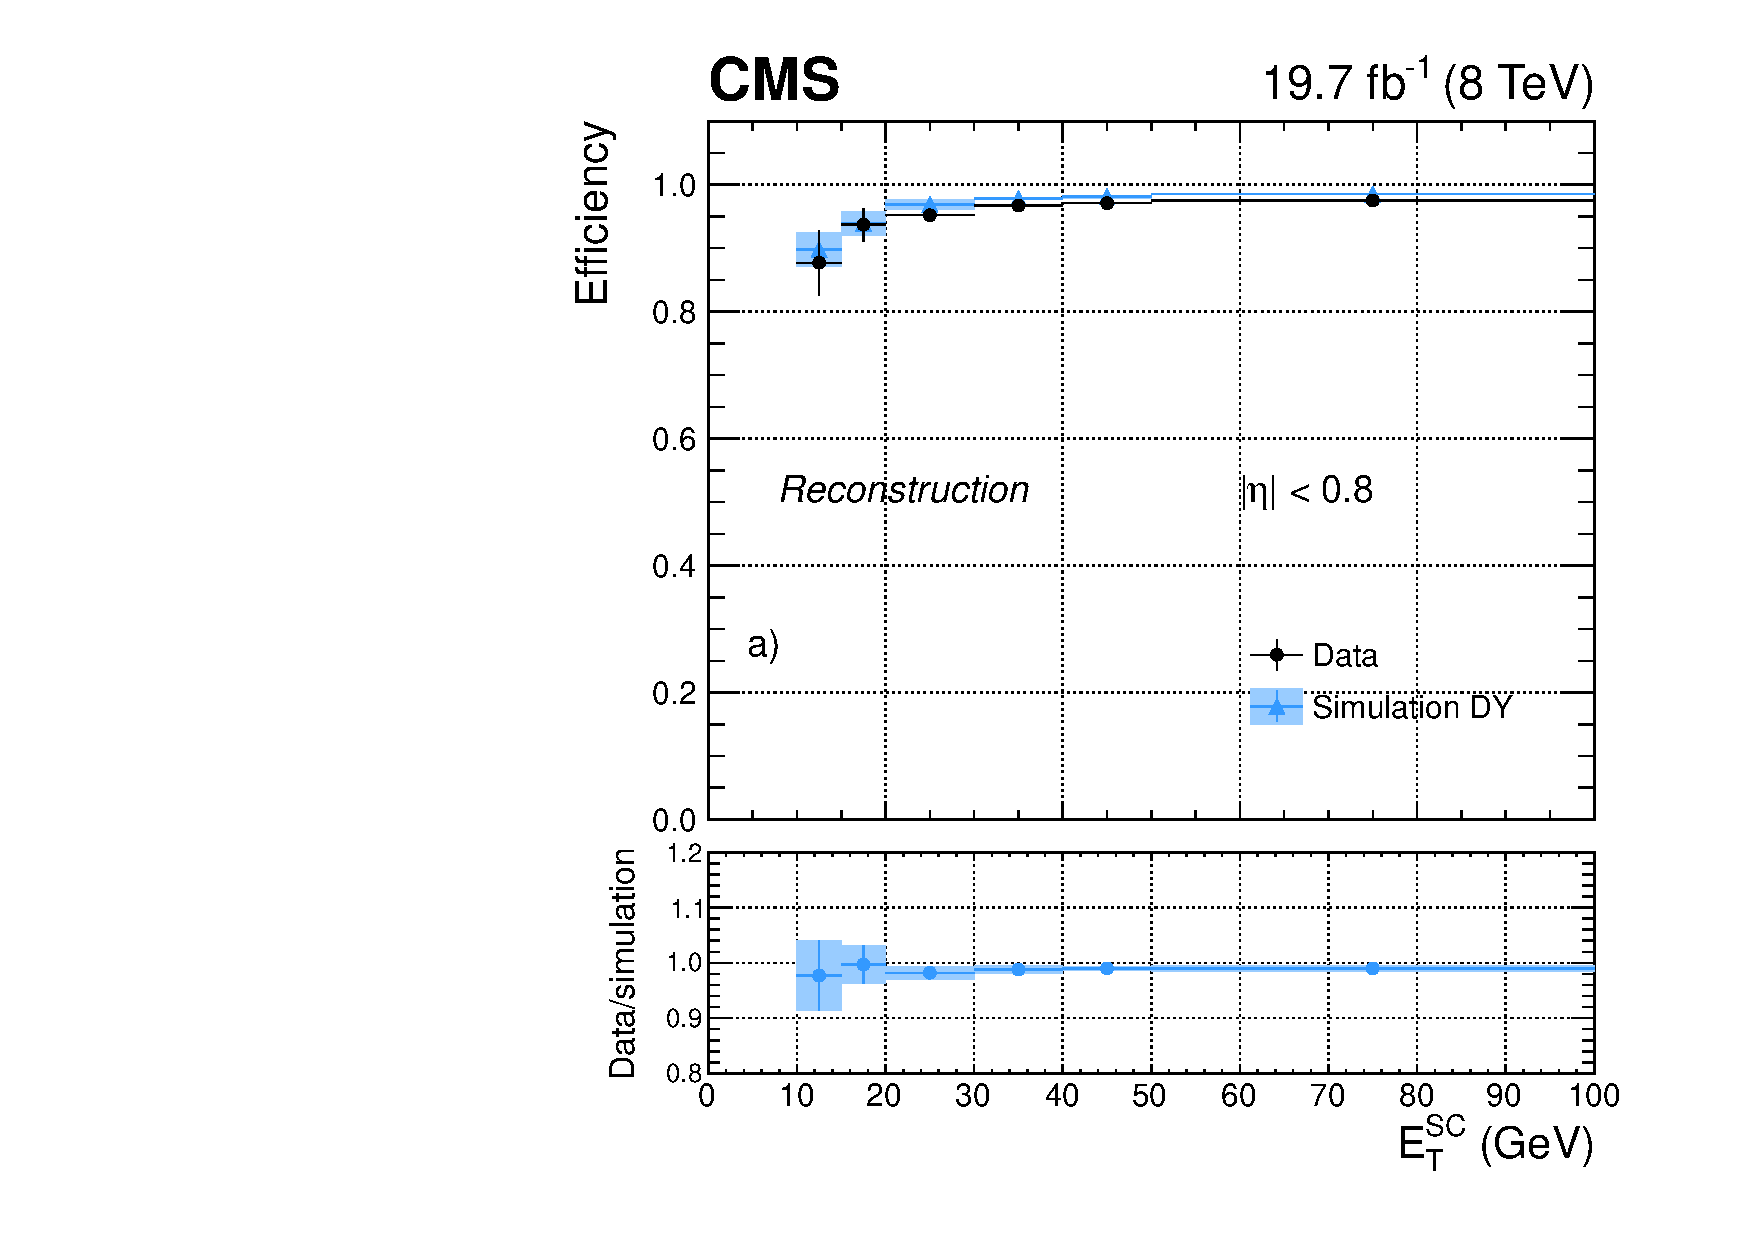
\includegraphics[width=0.45\textwidth]{\chsix/ele-reco-eff-eta-bin-0.pdf}}
\subfigure[]{\label{fig:el_reco_b}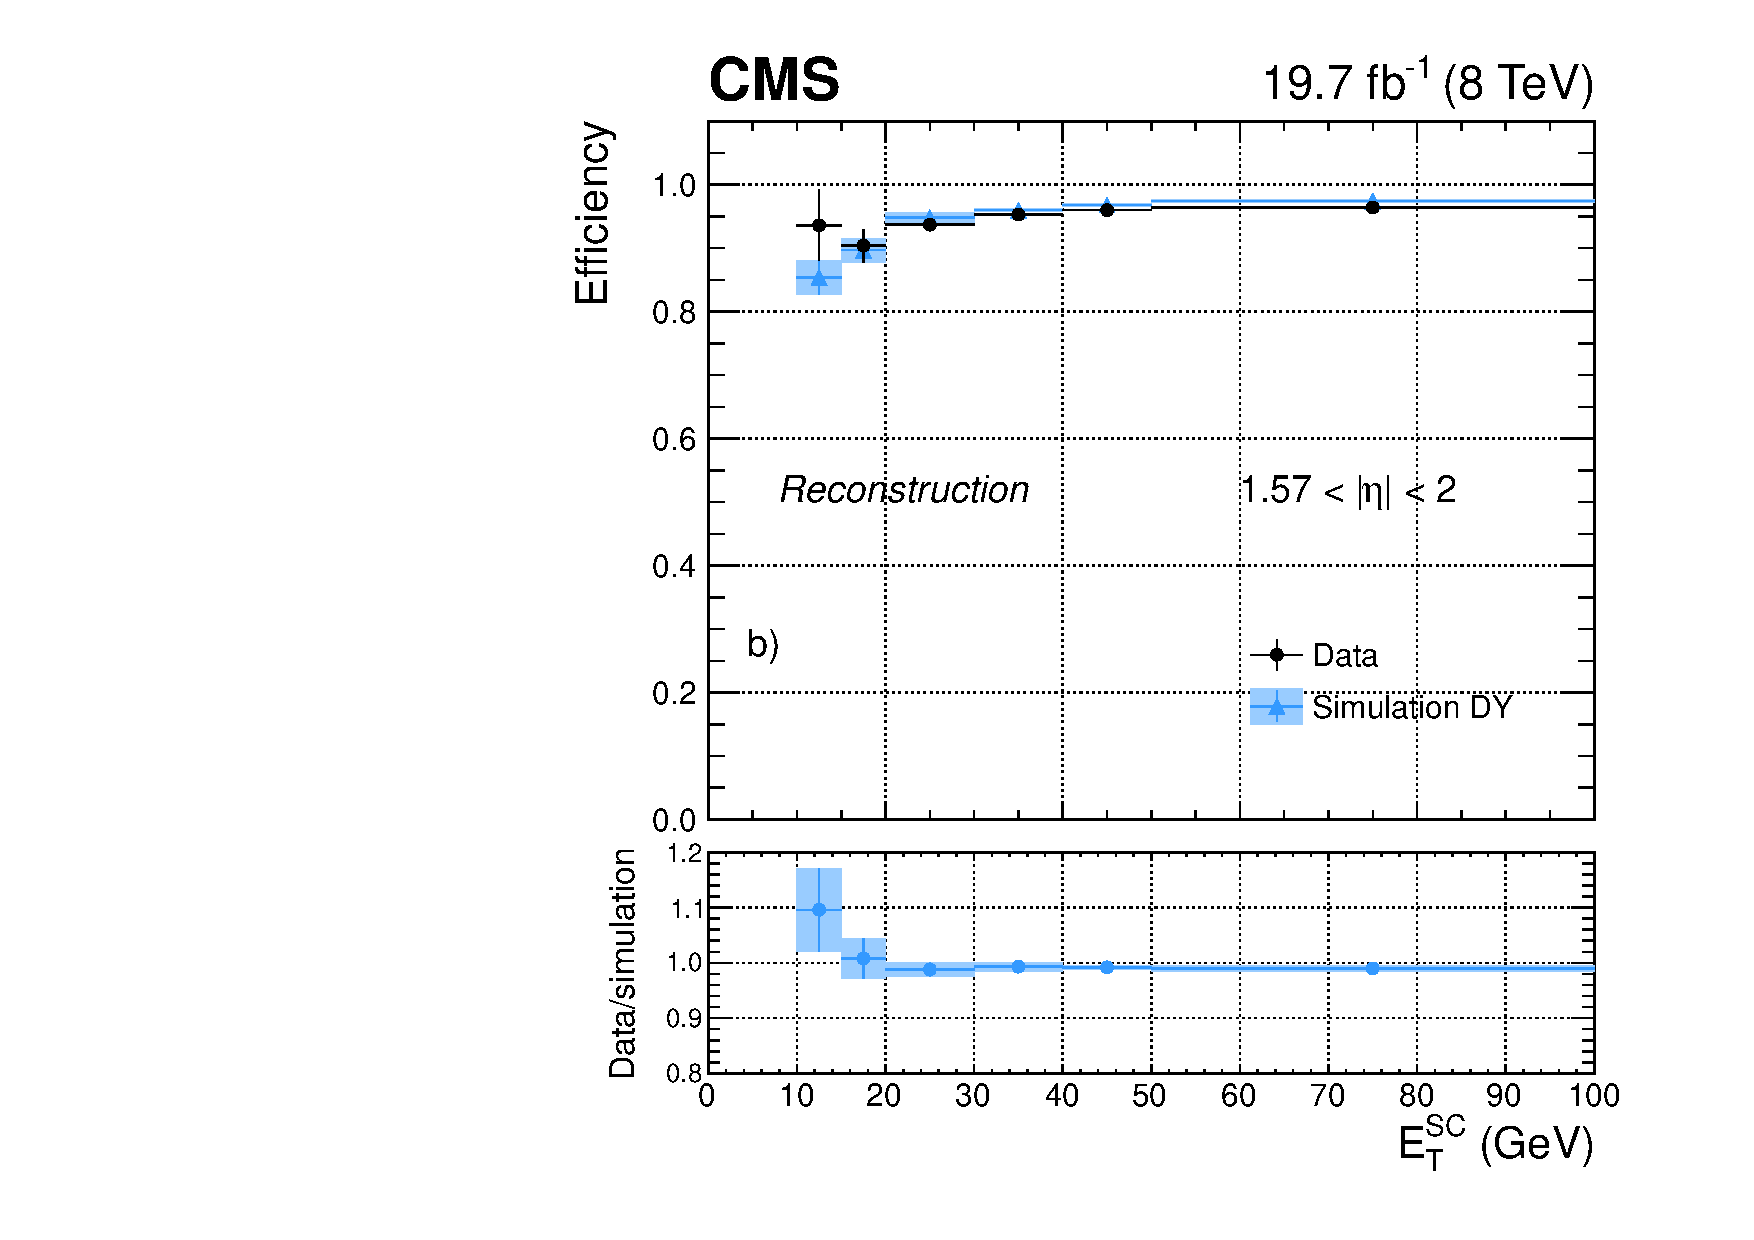
\includegraphics[width=0.45\textwidth]{\chsix/ele-reco-eff-eta-bin-3.pdf}}
\caption{Electron reconstruction efficiency measured in dielectron events in data (dots) and Drell-Yan simulation (triangles), as a function of the \et
for electrons reconstructed in the ECAL barrel (a) and endcaps (b). The bottom panels show the corresponding data-to-simulation scale factors~\cite{Khachatryan:2015hwa}.
%The uncertainties shown in the plots correspond to the quadratic sum of the statistical and systematic contributions~\cite{Khachatryan:2015hwa}.
}
\label{fig:el_reco}
\end{figure}

Once a GSF electron candidate is reconstructed, the energy measurement provided by electromagnetic calorimeter can be combined with the tracker momentum measurement to improve the estimate of electrons with energies below 35\GeV as shown in Fig.~\ref{fig:eleres}.
%For medium and low energy values ($< 35\GeV$), the momentum is obtained as a weighted sum of the supercluster energy and track momentum measurements.
At energies above 35\GeV however, the momentum measurement is completely driven by the supercluster.
%The energy measurement provided by electromagnetic calorimeter can be combined with the tracker momentum measurement to improve the estimate of the electron momentum for low energy particles. The improvement is expected to come both from the opposite behaviour with E or p of the intrinsic calorimetry and tracking resolutions, and from the fact that ptk and Esc are differently affected by the bremsstrahlung radiation (see Figure 2.12).

\begin{figure}[!htb]
 \begin{center}
  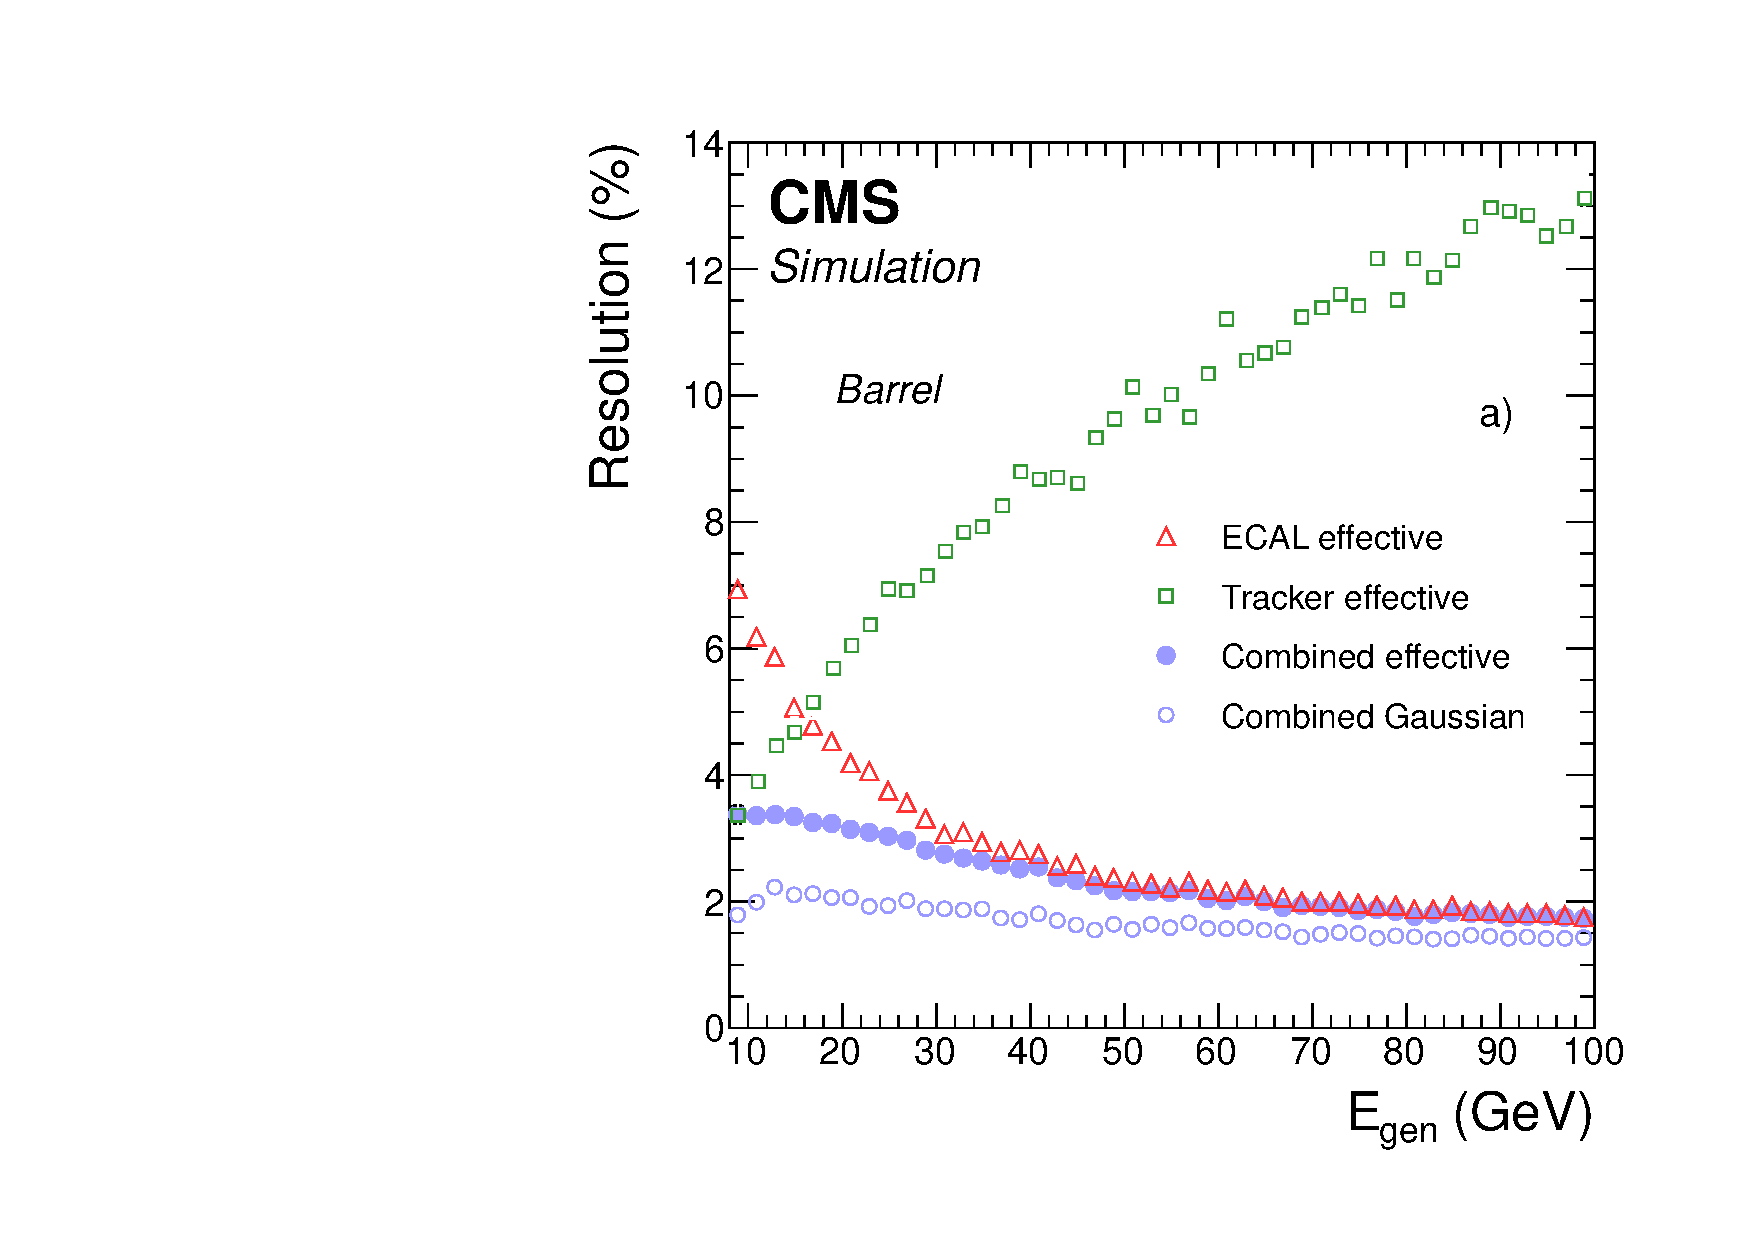
\includegraphics[width=0.45\textwidth]{\chsix/effRMSbarrel_withregression.pdf}
 \end{center}
 \caption{Expected resolution in \et for isolated electrons in the ECAL barrel as a function of the electron generated energy, obtained from the ECAL, the tracker and the combined estimates~\cite{Khachatryan:2015hwa}.}
 \label{fig:eleres}
\end{figure}

%%%%%%%%%%
\subsection{Electron trigger}\label{subsec:eletrigger}
%%%%%%%%%%

As explained in Section~\ref{subsec:CMStrigger}, the events of interest for physics analyses are selected by the trigger system in two steps, namely, the L1 and HLT.
%the trigger system consists of the layers: the Level 1 (L1) and the High Level Trigger (HLT).
At the L1, where the tracker information is not available, electrons and photons are indistinguishable and based on calorimeter trigger towers, consisting, in the barrel, of a $5\times5$ matrix of ECAL crystals and the corresponding HCAL tower, while a more complex definition of the tower is used in the endcaps. A L1 candidate is formed combining the highest-energy central trigger tower together with its next-highest adjacent tower.
At this stage, the trigger choice is based on the energy distribution among the central and neighbouring towers, on the amount of energy in the HCAL downstream the central tower, and on the \ET of the e/$\gamma$ candidate. 
%At this stage, the trigger choice is based only on the transverse energy of the calorimetric deposit, coarse shower shape requirements and the fraction of the total L1 seed energy belonging to the hadronic calorimeter, required to be smaller than 5\%.
%Two criteria on the shower shape are then applied: the ratio of the energy measured in the HCAL over the one in the ECAL is required to be less than 5\% and, in the barrel, 90\% of the ECAL energy must be contained in a 2 � 5 band of crystals in ? � ?. 
Events passing L1 are then filtered by the HLT. Here, the pixel tracker information is used to separate electrons from photons. The starting point of any electron HLT selection consists of building a supercluster and a trajectory as described in Section~\ref{subsec:elereco}. Many different triggers involving electrons are designed at the HLT level and various additional identification and isolation requirements on the electrons are made for each of them.
They consist of conditions on:

\begin{itemize}
\item transverse profile of the cluster of energy in the ECAL;
\item the amount of energy in the HCAL downstream the ECAL cluster;
\item the existence of a KF or GSF track matching the supercluster position;
\item quality of association between the track and the ECAL cluster;
\item activity in the ECAL, HCAL, or tracker around the candidate.
\end{itemize}

The conditions used and their severity depend on the number of electrons requested by the trigger and their transverse energy threshold, each trigger being designed to have a rate of accepting events of 50\unit{Hz} or less.
Practically, all the HLT steps and criteria involving only calorimeters information are done first, while the time consuming steps involving track reconstruction are only performed at the end for events passing the previous criteria.
The L1 and HLT triggers used to collect the data analyzed in this thesis are listed in Tables~\ref{tab:eletriggers8TeV} and~\ref{tab:eletriggers13TeV} for the 8 and 13\TeV data sets, respectively. The tables also detail the conditions imposed on several variables described in Section~\ref{subsec:eleid}.
Figure~\ref{fig:el_trig} shows the L1 trigger efficiencies for different \et thresholds as a function of the electron \et. The curves exhibit the typical turn on behaviour in correspondence of the imposed \et threshold.

\begin{table}[!htb]
\centering
\caption{The L1 and HLT single-electron triggers used to collect the 8\TeV data analyzed in this thesis together with the imposed requirements on the electron candidate.}
\resizebox{\textwidth}{!}{
\begin{tabular}{ l | c | c }
Trigger & Name & Selections\\
\hline
\hline
Level 1                     & L1\_SingleEG20                                                        & 1 e/$\gamma$ candidate \et $>$ 20 GeV\\
\hline
\multirow{6}{*}{HLT} & \multirow{6}{*}{HLT\_Ele80\_CaloIdVT\_GsfTrkIdT} & 1 GSF electron:\\
                                 &                                                                                   & \et $>$ 80\GeV\\
                                 &                                                                                   & $|\Delta\eta_{in}| < 0.008$\\
                                 &                                                                                   & $|\Delta\phi_{in}| < 0.07$ (barrel) or 0.05 (endcaps)\\
                                 &                                                                                   & $H/E < 0.05$\\
                                 &                                                                                   & $\sigma_{i\eta i\eta} < 0.011$ (barrel) or 0.031 (endcaps)\\
\end{tabular}}
\label{tab:eletriggers8TeV}
\end{table}

\begin{table}[!htb]
\centering
\caption{The L1 and HLT single-electron triggers used to collect the 13\TeV data analyzed in this thesis together with the imposed requirements on the electron candidate.}
\resizebox{\textwidth}{!}{
\begin{tabular}{ l | c | c }
Trigger & Name & Selections\\
\hline
\hline
\multirow{2}{*}{Level 1} & L1\_SingleEG35                                       & 1 e/$\gamma$ candidate \et $>$ 35 GeV\\
                                     & OR L1\_SingleEG40                                 & OR \et $>$ 40 GeV\\
\hline
\multirow{6}{*}{HLT}      &							             & 1 GSF electron:\\
                                     &   							     & \et $>$ 105\GeV OR $>$ 115\GeV\\
                                     & 	HLT\_Ele105\_CaloIdVT\_GsfTrkIdT	     & $|\Delta\eta_{in}| < 0.008$\\
                                     & 	OR HLT\_Ele115\_CaloIdVT\_GsfTrkIdT & $|\Delta\phi_{in}| < 0.07$ (barrel) or 0.05 (endcaps)\\
                                     & 							              & $H/E < 0.05$\\
                                     & 							              & $\sigma_{i\eta i\eta} < 0.011$ (barrel) or 0.031 (endcaps)\\
\end{tabular}}
\label{tab:eletriggers13TeV}
\end{table}

\begin{figure}[!htb]
\centering
\subfigure[]{\label{fig:el_trig_a}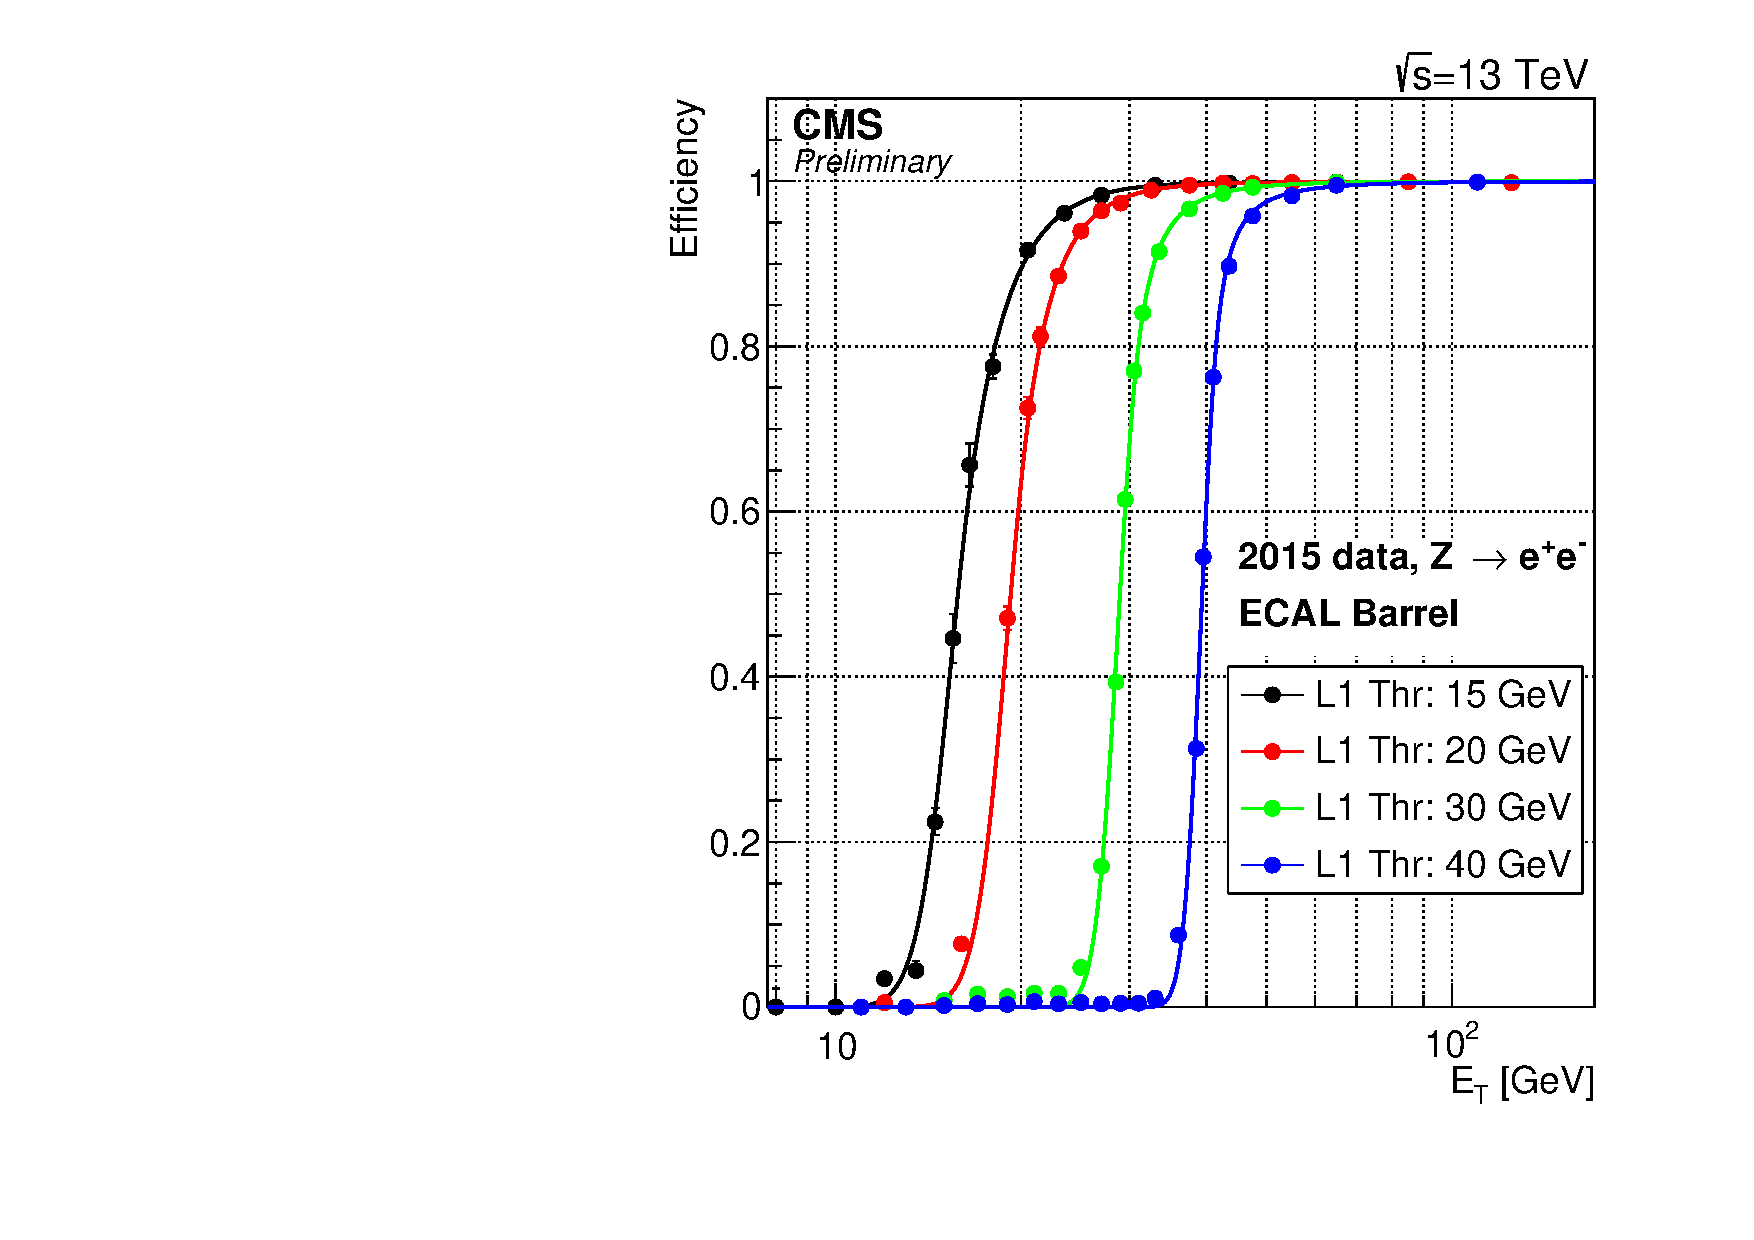
\includegraphics[width=0.45\textwidth]{\chsix/plot_iEG_2015.pdf}}
\subfigure[]{\label{fig:el_trig_b}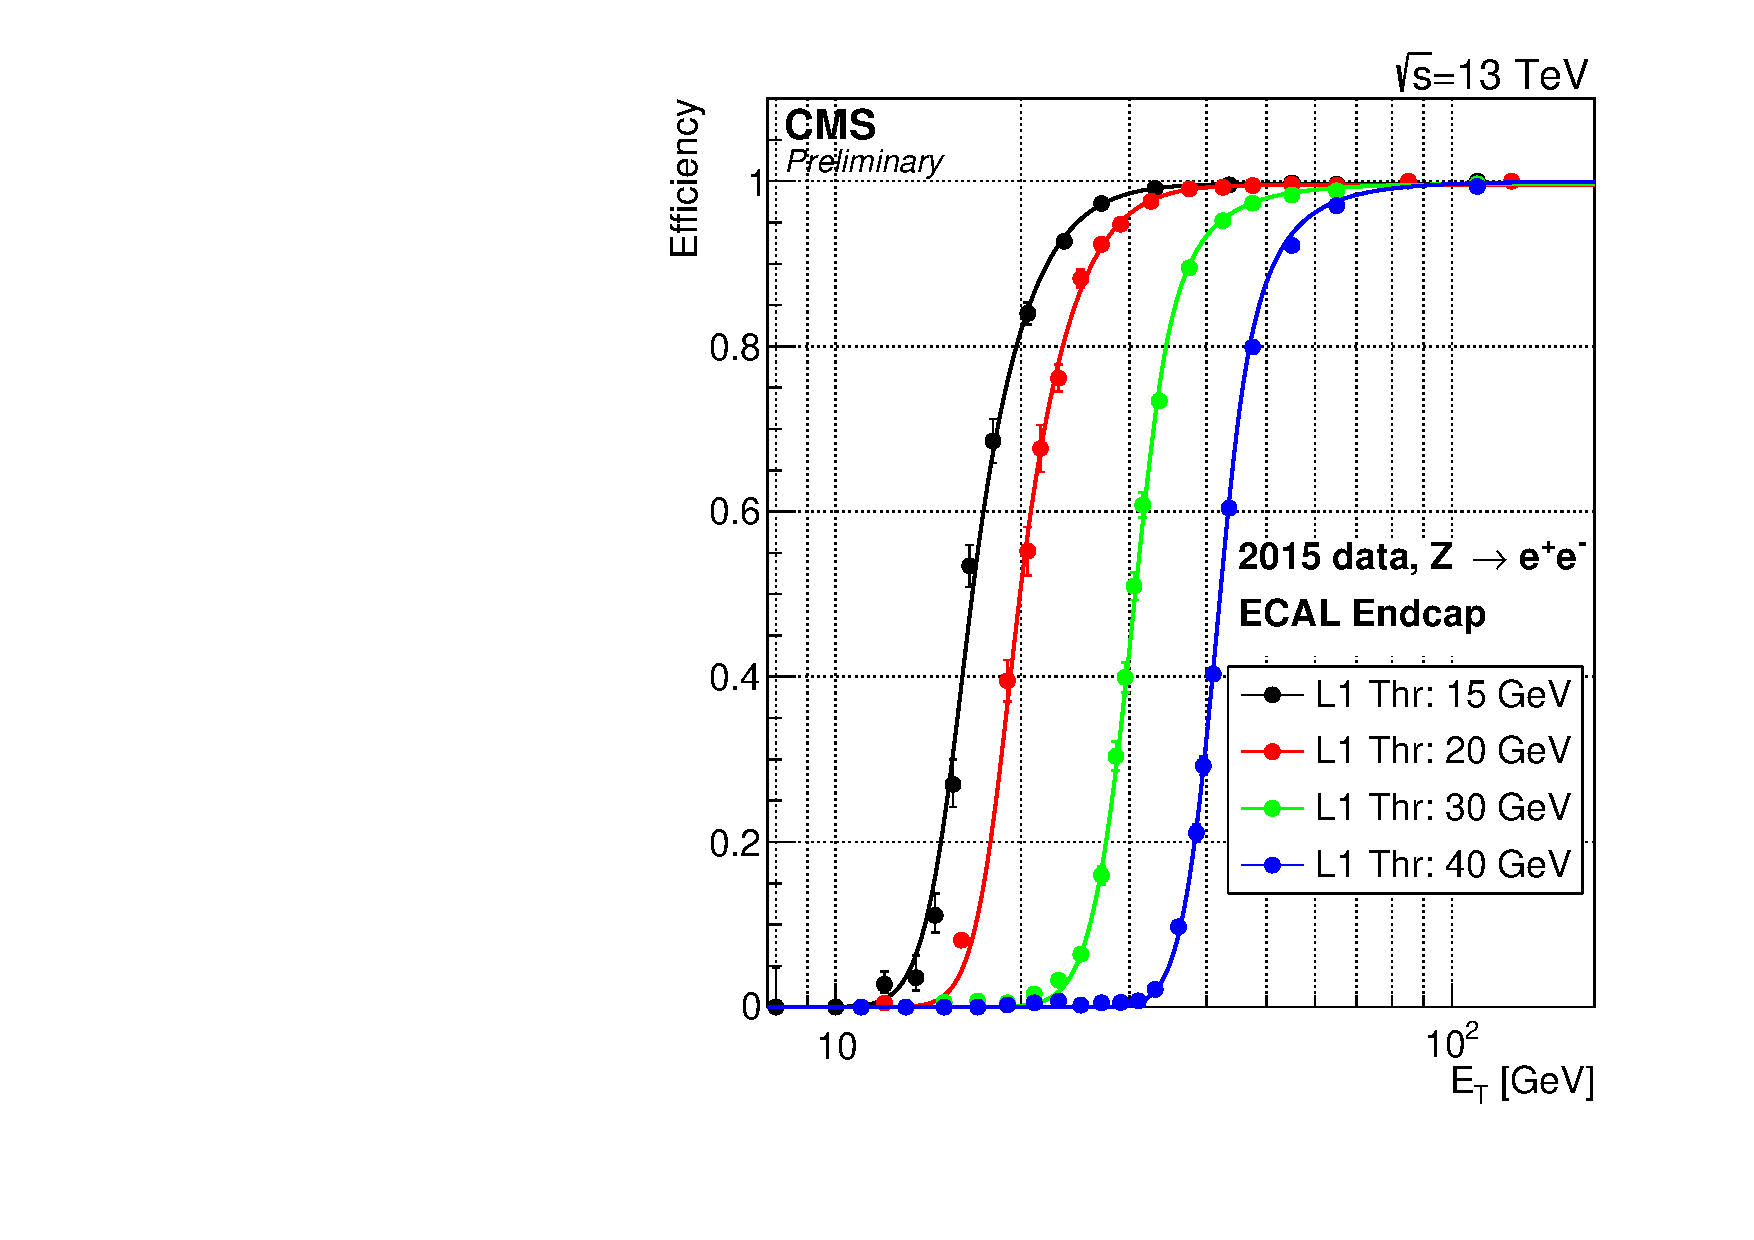
\includegraphics[width=0.45\textwidth]{\chsix/plot_EE_iEG_2015.pdf}}
\caption{L1 electron triggering efficiency in ECAL barrel (a) and endcaps (b) as a function of the offline reconstructed electron \et. The efficiency is shown for the 15, 20, 30, 40\GeV EG trigger thresholds~\cite{ECALPublicResults}.}
\label{fig:el_trig}
\end{figure}

Both the L1 and HLT triggers require one electron (or $\gamma$) candidate.  
The \et thresholds imposed for the data collected in pp collisions at 13\TeV are higher compared to the one used in Run~1, in order to keep low trigger rates given the higher production rates of low-energy multijet background expected in Run~2. The chosen HLT triggers require a reconstructed GSF track whose association to the ECAL cluster has to pass tight quality criteria ($|\Delta\eta_{in}|$ and $|\Delta\phi_{in}|$).
Requirements are also applied at this level on the transverse profile of the cluster of energy in the ECAL ($\sigma_{i\eta i\eta}$) and on the amount of energy in the HCAL downstream the ECAL ($H/E$). There are no requirements imposed on the electron candidate isolation. 
In general, this results in high fake rates of jets misreconstructed as electrons from multijet background, and, as a consequence, in high trigger rates which would require a prescale. However, the high \et threshold allows for an unprescaled trigger, as jets from multijet background are characterized by low momentum. In addition, the kinematic region of the analyses presented in this thesis is located at very high lepton \pt and the signal efficiency is mainly affected at very low resonance masses ($< 1\TeV$) with a loss in efficiency of 20--25\%.\\
%The offline reconstructed \pt of the electrons must be greater than 90 (120) \GeV for the 8 (13) TeV analysis, where the trigger reaches the plateau. In fact, this choice is made to simplify the analysis avoiding the need for modelling the trigger turn-on curve and, as a consequence, reducing the associated systematic uncertainties.

The efficiency for an electron passing the high-\et selections described in Sec.~\ref{subsec:eleid} to fire the HLT triggers of Tables~\ref{tab:eletriggers8TeV} and \ref{tab:eletriggers13TeV} have been measured in data with T\&P method and are found to be 98-99\% for electrons with \et in the trigger plateau, with data-to-simulation scale factors close to unity.
%The efficiency for a HEEP electron to pass the HLT_Ele105 are 0.984 (barell) 0.998 (endcap) in the plateau. For HLT115 are 0.971/0.966. (W' analysis AN-2015/226)
%from W'->l+MET 8 TeV: The trigger efficiency for single electrons has been determined with ?tag-and-probe? methods [65] to be 99.1 (97.6)% for the barrel (endcap) ECAL, with a data-to-simulation scale factor of nearly one. (https://arxiv.org/pdf/1408.2745v2.pdf)

%%%%%%%%%%
\subsection{Electron identification}\label{subsec:eleid}
%%%%%%%%%%

All the physics analyses in CMS involving one or two electrons in the final state start with the general electron reconstruction algorithm presented in Section~\ref{subsec:elereco}.
%The electron reconstruction presented in Section~\ref{subsec:elereco} is the starting point of any electron selection in CMS and it is used by any physics analysis involving one or several electrons in the final state.
A high efficiency in any kinematical conditions is therefore needed and, as a consequence, the probability for other particles to be reconstructed as electrons is sizeable.
For instance, a charged pion can mimic the signature of an electron if it interacts early and leaves most of its energy in the ECAL. Moreover electrons can emerge in a jet through the weakly decay of a hadron containing a c or b quark. Finally, in addition to jets, photons can also lead to GSF electron candidates. This happens if the photon converts into a dielectron pair in one of the first layers of the tracker detector. If one of the electron takes most of the photon momentum, a GSF electron candidate is likely to be reconstructed.
%In fact, the GSF electron candidates reconstructed in the data are mainly other physics objects misreconstructed as electrons, or ``fakes''. These fakes are of several kinds: a charged pion can for instance mimic the signature of an electron if it interacts early and leaves most of its energy in the ECAL. Moreover electrons can emerge in a jet through the weakly decay of a hadron containing a c or b quark. Finally, in addition to jets, photons can also lead to GSF electron candidates. This happens if the photon converts into a dielectron pair in one of the first layers of the tracker detector. If one of the electron takes most of the photon momentum, a GSF electron candidate is likely to be reconstructed.
An analysis dependent selection, which takes into account the specific kinematics and background level, has therefore to be applied on top of the electron reconstruction. This thesis focuses on the search for massive resonances decaying to pairs of SM bosons where one of the bosons is a W decaying leptonically, with a highly energetic electron or muon in the final state. A high and stable selection efficiency for \et above 100\GeV is therefore an important requirement.
%Most of the searches for new physics involving high energy electrons share the same features:
%-The cross sections probed are tiny (sometimes below 1 fb).
%-The background due to jets or other particles wrongly reconstructed as GSF electron candidates is moderate.
%-The electron energy range under study is large (from ET = 100 GeV to ? 1 TeV).
%-The usual control region to check the performance of an electron selection in the data is the Z peak, where a large statistics is available for electrons with ET ? 35 GeV.
%-For higher ET values, the control regions (events with boosted on-shell Z or high mass tail of the Drell-Yan process) suffer from low statistics.
%A high and stable selection efficiency for ET above 100GeV is therefore the main requirement. The selection must also reasonably work for lower values, down to 35 GeV. Finally, given the fact that the validation of the selection at high ET in data is difficult, a simple and understandable selection is preferred.
Since this is a common feature of many searches for new physics, a specific cut based selection has been developed in CMS~\cite{Khachatryan:2014fba}, consisting of requirements on several variables that exploit the characteristics of high-\et electrons. Only GSF electron candidates with $\et > 35\GeV$ and well reconstructed in the tracker and ECAL sensitive regions are selected. Candidates in the ECAL transition region ($1.442 < |\eta_\mathrm{SC}| < 1.56$) and beyond the $\eta$ coverage ($|\eta_\mathrm{SC}|  > 2.5$) of the tracker are therefore discarded. A different selection is applied for candidates reconstructed in the ECAL barrel ($|\eta_\mathrm{SC}| < 1.442$) and endcaps ($1.56 < |\eta_\mathrm{SC}|  < 2.5$). For Run~2 the values of $\eta_\mathrm{SC}$ have been slightly adjusted to match the acceptance of the detector more accurately. The selections are summarized in Tables~\ref{tab:heep8TeV} and \ref{tab:heep13TeV}, for the 8 and 13\TeV data analysis, respectively, and discussed in the following.

%https://twiki.cern.ch/twiki/bin/viewauth/CMS/HEEPElectronID
\begin{table}[!htb]
\centering
\caption{List of the variables used in the high-\et electron selections for the 8\TeV data analysis, together with the corresponding requirements for electrons reconstructed in the ECAL barrel and endcaps.}
\resizebox{\textwidth}{!}{
\begin{tabular}{ l | c | c }
Variable & ECAL barrel & ECAL endcaps\\
\hline
\hline
ECAL-driven & yes & yes\\ 
\et & $> 35\GeV$ & $> 35\GeV$\\
$|\eta_{\mathrm SC}|$ & $< 1.442$ & 1.56--2.5\\
$|\Delta\eta_{in}|$ & $< 0.005$ & $< 0.007$\\
$|\Delta\phi_{in}|$ & $< 0.06$ & $< 0.06$\\
Relative track isolation & 5\% & 5\% \\
\multirow{2}{*}{Calorimeter isolation} & \multirow{2}{*}{$< 2 + 0.03\et +0.28\rho$} & $< 2.5 + 0.28\rho$ if $\et < 50$\\
 & & $< 2.5 + 0.03(\et-50) + 0.28\rho$ if $\et \geq 50$\\  
\multirow{2}{*}{Transverse shower shape} & $E_{2\times5}/E_{5\times5} > 0.94$ & \multirow{2}{*}{$\sigma_{i\eta i\eta} < 0.03$} \\
  & OR $E_{1\times5}/E_{5\times5} > 0.83$ & \\
%$\sigma_{i\eta i\eta}$ & - & $< 0.03$\\
$H/E$ & $< 0.05$ & $< 0.05$\\
$|d_{xy}|$ & $< 0.02$ & $< 0.05$\\
Inner layer lost hits & $\leq 1$ & $\leq 1$\\
\end{tabular}}
\label{tab:heep8TeV}
\end{table}

\begin{table}[!htb]
\centering
\caption{List of the variables used in the high-\et selections for the 13\TeV data analysis, together with the corresponding requirements for electrons reconstructed in the ECAL barrel and endcaps.}
\resizebox{\textwidth}{!}{
\begin{tabular}{ l | c | c }
Variable & ECAL barrel & ECAL endcaps\\
\hline
\hline
ECAL-driven & yes & yes\\ 
\et & $> 35\GeV$ & $> 35\GeV$\\
$|\eta_{\mathrm SC}|$ & $< 1.4442$ & 1.566--2.5\\
$|\Delta\eta_{in}|$ & $< 0.004$ & $< 0.006$\\
$|\Delta\phi_{in}|$ & $< 0.06$ & $< 0.06$\\
Relative track isolation & 5\% & 5\% \\
\multirow{2}{*}{Calorimeter isolation} & \multirow{2}{*}{$< 2 + 0.03\et +0.28\rho$} & $< 2.5 + 0.28\rho$ if $\et < 50$\\
 & & $< 2.5 + 0.03(\et-50) + 0.28\rho$ if $\et \geq 50$\\  
\multirow{2}{*}{Transverse shower shape} & $E_{2\times5}/E_{5\times5} > 0.94$ & \multirow{2}{*}{$\sigma_{i\eta i\eta} < 0.03$} \\
  & OR $E_{1\times5}/E_{5\times5} > 0.83$ & \\
%$\sigma_{i\eta i\eta}$ & - & $< 0.03$\\
$H/E$ & $< 1/E + 0.05$ & $< 5/E + 0.05$\\
$|d_{xy}|$ & $< 0.02$ & $< 0.05$\\
Inner layer lost hits & $\leq 1$ & $\leq 1$\\
\end{tabular}}
\label{tab:heep13TeV}
\end{table}
%https://twiki.cern.ch/twiki/bin/view/CMS/HEEPElectronIdentificationRun2#Selection_Cuts_HEEP_V6_0_Recomme

As a starting point, electrons are selected if the reconstruction was seeded in the ECAL (Section~\ref{subsec:elereco}). In fact, while useful for low-energy and non-isolated electrons, the PF algorithm is less suitable for high-energy electrons.

%deltaEta/deltaPhi in
The difference in $\eta$, $\Delta\eta_{in}$, and in $\phi$, $\Delta\phi_{in}$, between the track position as measured in the inner layers, extrapolated to the interaction vertex and to the calorimeter, and the position of the supercluster, are required to be $< 0.005$ and $< 0.06$, respectively. In fact, for jets, the position of the center of the ECAL deposit can be far from the track position, as all of the constituents can leave an energy deposit in the ECAL. The $\Delta\phi_{in}$ distribution is however much broader than $\Delta\eta_{in}$, because of the wider spread of the energy in $\phi$ due to photons from bremsstrahlung, resulting in a looser requirement. The distributions of $\Delta\phi_{in}$ and $\Delta\eta_{in}$ become narrower with increasing \et, and therefore a higher discrimination power can be achieved with a tighter requirement at high \et compared to the usual selections for low or intermediate energetic electrons. The reason of this behaviour comes from the fact that bremsstrahlung photons are more collinear to the electron at higher \et. The definition of $\Delta\eta_{in}$ has been changed for Run~2 to use instead the $\eta$ of the seed cluster of the supercluster which is found to provide a more accurate indication of the $\eta$ of the original electron before bremsstrahlung. 

%trackIso
To suppress the misidentification of jets as electrons, the sum of the \pt of all other tracks in a cone of $\Delta R < 0.3$ around the track of the electron candidate is required to be less than 5\GeV, imposing an isolation condition on the electron candidate track. To be used in the calculation of the isolation of the candidate track, the tracks have to be within 0.2\cm, in the $z$ direction, of the primary vertex with which the electron candidate is associated. This requirement reduces the impact of pileup and it does not show a dependency with the electron \et for values above 100\GeV.
%For electrons with transverse energies above 100\GeV, a negligible change in the selection efficiency is observed as the number of pileup events increases from 0 to 40.
For electrons with \et much lower than 100\GeV, the efficiency decreases up to 10\% depending on the region of the detector in which the electrons are detected. 

%ECAL+HCAL1 iso
A calorimeter-based isolation is applied and defined as the sum of:

\begin{itemize}
\item ECAL isolation: sum of the \et of the energy deposits in the ECAL calorimeter in a cone of $\Delta R < 0.3$ around the track of the electron candidate excluding those associated with the candidate;
\item HCAL1 isolation: sum of the \et of the energy deposits in the first layer of the HCAL calorimeter in a cone of $\Delta R < 0.3$ around the track of the electron candidate excluding those associated with the candidate.
\end{itemize}

The isolation variable so defined, is required to be less than 3\% (plus a small $\eta$-dependent offset) of the candidate \et.
%Within this same cone, the sum of the \et of the energy deposits in the calorimeter that are not associated with the candidate is required to be less than 3\% (plus a small $\eta$-dependent offset) of the candidate \et.
This sum, which allows a selection on the isolation of the electron candidate, is corrected for the average energy density in the event, $\rho$, to minimize the dependence of the efficiency of this selection criterion on pileup. 
This requirement differs from the selection usually applied for electrons of low or intermediate \et. For these cases, a PF-based isolation is generally used, which merges the information of the tracker, the ECAL and the HCAL allowing to measure the contribution to the isolation from charged hadrons, neutral hadrons and photons separately. One of the main advantage of the PF-based isolation is that the energy deposit in the calorimeters associated to a charged hadron produced in another interaction, characterized by a different primary vertex, can be removed from the isolation sum. For very high energy ($ > 1\TeV$) electrons, however, the PF algorithm might fail to recognize an electron from a GSF electron candidate and assigns all its energy deposit to the photon isolation. 
Furthermore, the PF isolation is generally required to be below a fixed fraction of the electron \et independently on its value.
However, for high \et values the background rejection can be improved while keeping an acceptable efficiency by following the \et dependence of the ECAL+HCAL1 isolation variable.
In fact, this isolation tends to increase for high-\et electrons due to the extension of the shower.
%To better follow the ET evolution and hence improve the background rejection while keeping an acceptable efficiency at moderate ET the HEEP cut value is of the form Iso < A + B � ET . 
%This requirement is suitable for electrons with \et in the low or intermediate range ($\et < 50--100\GeV$) but it results in a very loose selection for electrons with much higher \et (150\GeV for $\et = 1\TeV$).
%This is perfectly acceptable at moderate ET (ET < 50-100 GeV) but this would mean a cut value of 150 GeV for an electron with ET = 1 TeV which is far above the typical values for real electrons.

%H/E + profile
Further suppression of the misidentification of jets as electrons is
achieved by requiring that the ratio $H/E$ of the energy in the HCAL towers in a cone of $\Delta R < 0.15$ centered on the electron candidate position, to the electromagnetic energy of the electron candidate supercluster is required to be less than 5\%. This requirement is tighter compared with the threshold applied for low- or medium-energy electrons, where it becomes quite inefficient for a high number of pileup interactions.
%where the contribution from pileup. Therefore, a weaker selection is applied to avoid large signal inefficiencies.
For Run~2, the selection on this variable has been increased.
Additionally, the transverse profile of the energy deposition in the ECAL is required to be consistent with that expected for an electron, being defined by the following variables:

\begin{itemize}
\item $E_{1\times5}/E_{5\times5}$: ratio of the energy contained in the 1$\times$5 matrix in $\eta\times\phi$ in the barrel ($x\times y$ in the endcaps) centered on the seed crystal of the supercluster over the energy of the $5\times5$ matrix centered on the seed crystal;
\item $E_{2\times5}/E_{5\times5}$: ratio of the energy contained in the most energetic 2$\times$5 matrix in $\eta\times\phi$ in the barrel ($x\times y$ in the endcaps) centered on the seed crystal of the supercluster over the energy of the $5\times5$ matrix centered on the seed crystal;
\item $\sigma_{i\eta i\eta}$ : measure of the spread in $\eta$ in units of crystals of the electrons energy in the $5\times5$ block centered on the seed crystal.
\end{itemize}

In the barrel, the best performance are obtained applying a selection on both $E_{1\times5}/E_{5\times5}$ and $E_{2\times5}/E_{5\times5}$.
The two variables are indeed complementary: while $E_{1\times5}/E_{5\times5}$ is well designed for electrons hitting the center of a crystal, $E_{2\times5}/E_{5\times5}$ allows to recover electrons that hit the crystal close to its edge. Combining the two variables instead of using just one of them allows to set a  tight requirement on both and thus well reject background while keeping a high efficiency on simulated electrons. 
The distributions of these variables are much broader for electrons in the endcaps and a higher discrimination power is obtained applying a selection on the variable $\sigma_{i\eta i\eta}$.
%This is because the x ? y geometry does not follow the ? ? ? direction. As a consequence, part of the energy is sometimes missing in both E1�5/E5�5 and E2�5/E5�5 and their discrimination power is reduced and becomes worse than ?i?i?.
%H/E
%The cut value (0.05) is sensibly lower than the one usually used at moderate ET (0.12 in the barrel and 0.10 in the endcaps). At moderate ET this cut is indeed quite inefficient for a high number of pile-up interactions in the event ... why?

%missing hits + dxy
Two additional requirements are applied to reject photons that convert into a electron-positron pair in the tracker.
First, the track associated with the cluster is required to have no more than one hit missing in the pixel layers.
%It is mainly designed to reject photons that convert into a pair in the tracker as can be seen from figure 4.14. It can happen that only one of the electron tracks is reconstructed.
IN fact, the signature arising from photon conversion process is very similar to the one from real electrons, and the gain in discrimination using shower shape variables is limited. However, one of the main differences is the absence of hits in the first layers of the tracker, before the conversion happens.
Furthermore, the transverse impact parameter $d_{xy}$, defined as the closest distance, in the transverse plane, between the primary vertex and the track of the electron candidate, is required to be $< 0.02\cm$ (barrel) or 
$0.05\cm$ (endcaps). The distribution of the transverse impact parameter is usually wider in the endcaps due to the poorer resolution of the track position in that region.\\

The efficiency of the high-\et electron selection measured with the T\&P method in pp collisions at $\sqrt{s} = 8\TeV$ and in simulation as a function of the electron \pt is shown in Fig.~\ref{fig:el_heep}, for electrons reconstructed in the ECAL barrel and endcaps. Similar results are obtained using 13\TeV data. The efficiencies and data-to-simulation scale factors are summarized in Tables~\ref{tab:heepsf8TeV} and~\ref{tab:heepsf13TeV}, as measured in 8 and 13\TeV data and simulation, respectively. The scale factors are close to unity, indicating a good agreement between data and simulation. They are used in the analysis presented in this thesis to correct the normalization of simulations.

\begin{figure}[!htb]
\centering
\subfigure[]{\label{fig:el_heep_a}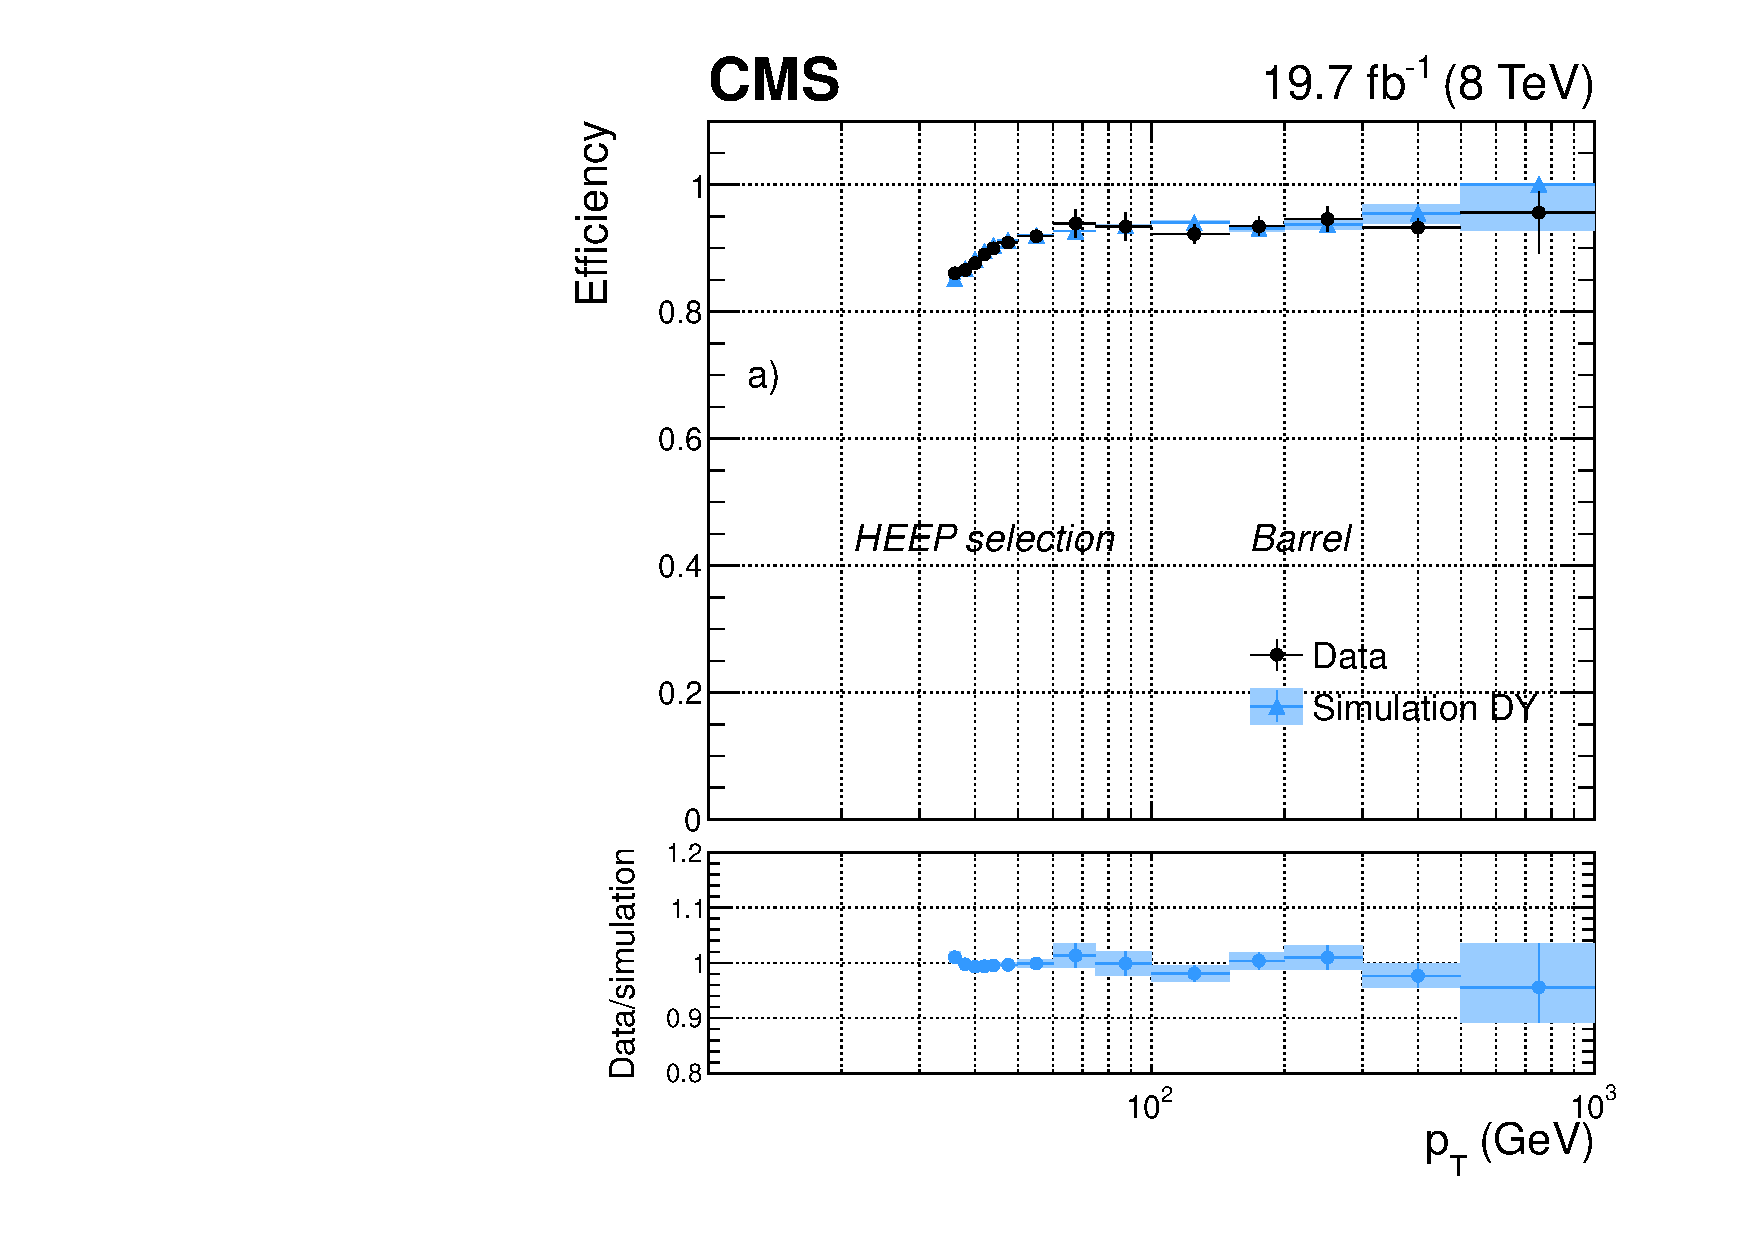
\includegraphics[width=0.45\textwidth]{\chsix/HEEPSF_barrel.pdf}}
\subfigure[]{\label{fig:el_heep_b}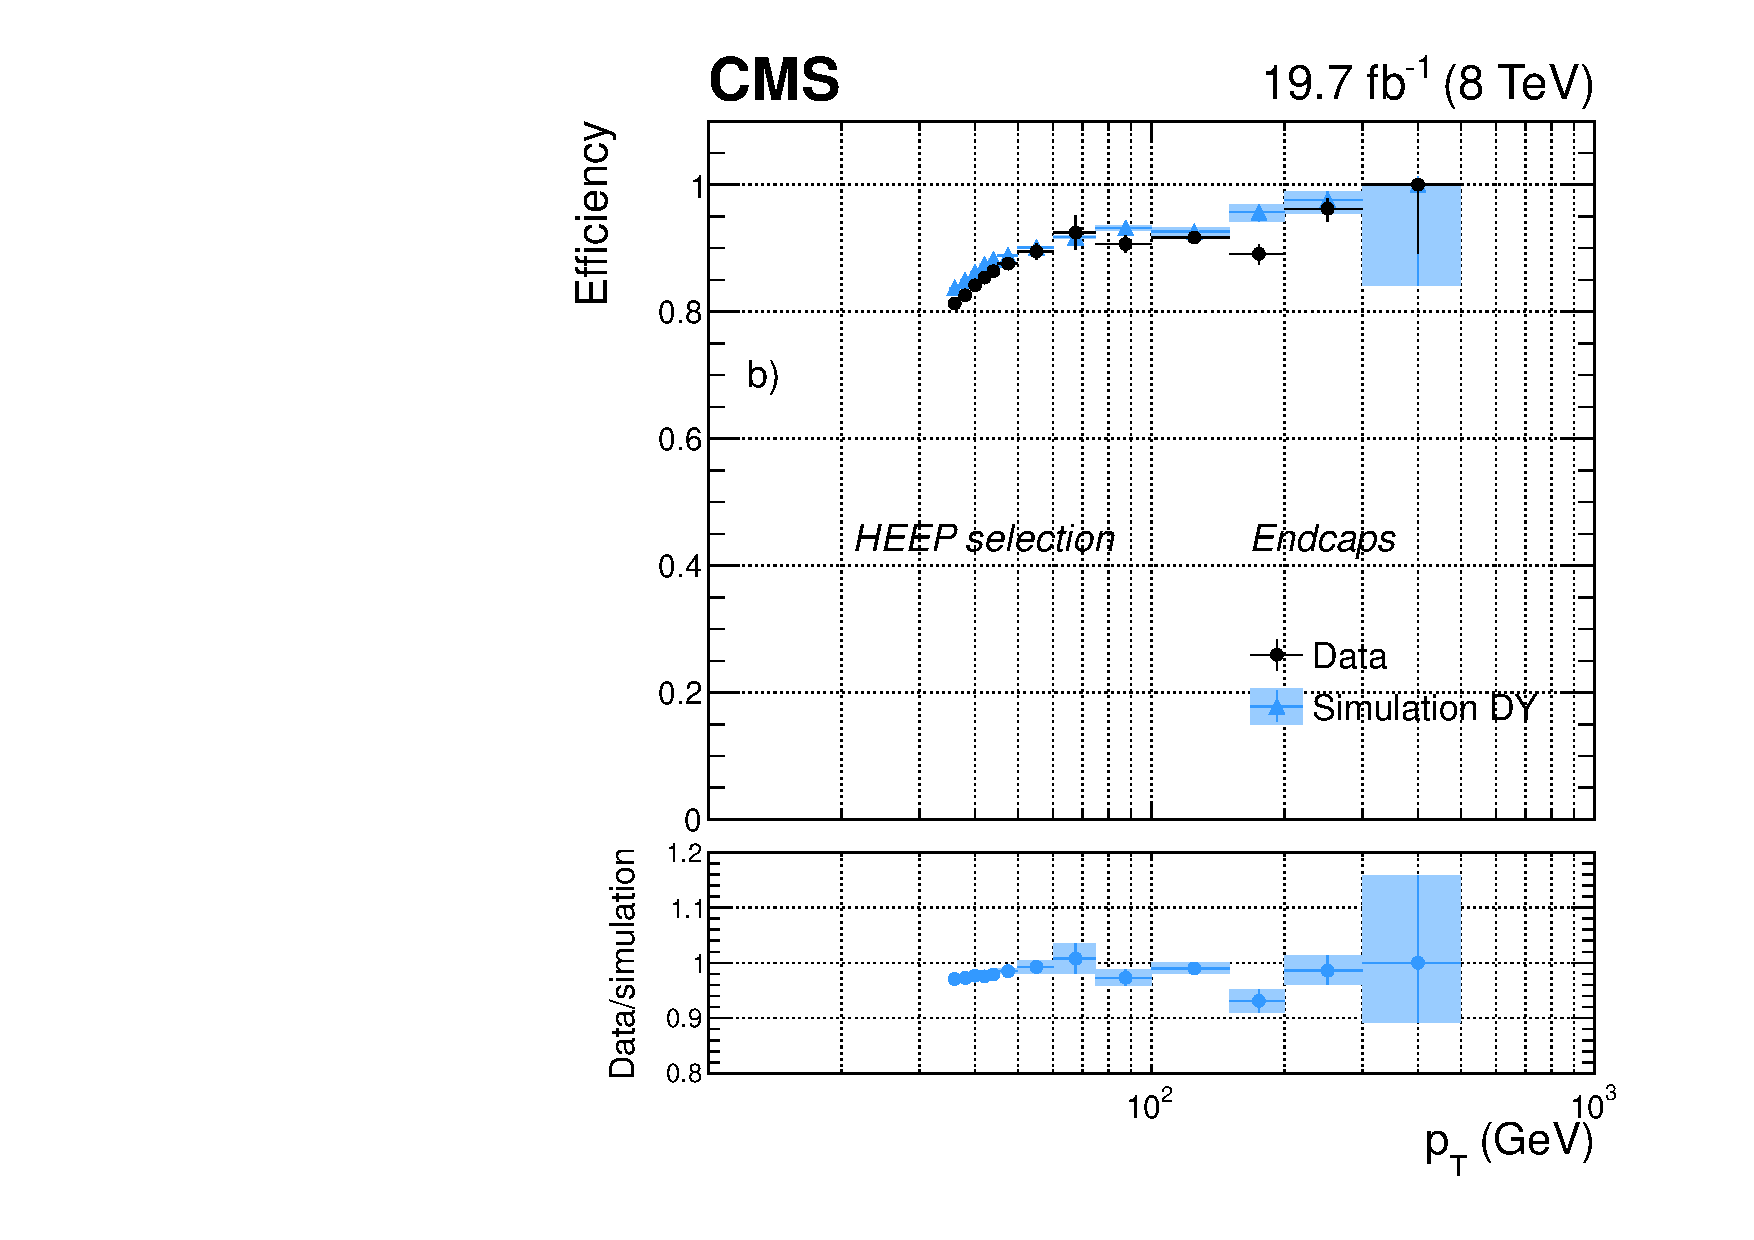
\includegraphics[width=0.45\textwidth]{\chsix/HEEPSF_endcaps_corr_noeffgt1.pdf}}
\caption{Efficiency of the high-\et electron selection as a function of electron \pt for dielectron events in pp collisions at $\sqrt{s} = 8\TeV$ (dots) and in DY simulation (triangles) for electrons reconstructed in the ECAL barrel (a), and endcaps (b)~\cite{Khachatryan:2015hwa}.}
\label{fig:el_heep}
\end{figure}

\begin{table}[!htb]
\centering
\caption{Efficiencies and data-to-simulation scale factors for the high-\et electron selection, as measured in pp collisions at $\sqrt{s} = 8\TeV$ for electrons with $\et > 90\GeV$. The quoted uncertainties are statistical.}
\begin{tabular}{ c | c | c}
 & ECAL barrel & ECAL endcaps\\
\hline
\hline
Efficiency simulation & 90.2\% $\pm$ 0.2\% & 92.2\% $\pm$ 0.5\%\\
Efficiency data & 88.7\% $\pm$ 0.2\% & 90.7\% $\pm$ 0.6\%\\
Data/simulation scale factor & 0.983 $\pm$ 0.004 & 0.984 $\pm$ 0.010 \\
\hline 
\end{tabular}
\label{tab:heepsf8TeV}
\end{table}
%https://twiki.cern.ch/twiki/bin/viewauth/CMS/HEEPEfficiencies#Efficiencies_and_scale_factors_f

\begin{table}[!htb]
\centering
\caption{Efficiencies and data-to-simulation scale factors for the high-\et electron selection as measured in pp collisions at $\sqrt{s} = 13\TeV$ for electrons with $\et > 120\GeV$. The quoted uncertainties are statistical.}
\begin{tabular}{ c | c | c}
 & ECAL barrel & ECAL endcaps\\
\hline
\hline
Efficiency simulation & 91.4\% $\pm$ 0.10\% & 84.4\% $\pm$ 0.3\%\\
Efficiency data & 91.6\% $\pm$ 0.04\% & 82.3\% $\pm$ 0.1\%\\
Data/simulation scale factor & 1.002 $\pm$ 0.001 & 0.975 $\pm$ 0.004\\
\hline 
\end{tabular}
\label{tab:heepsf13TeV}
\end{table}
%from Z'->ll AN-2015/222
